\documentclass[a4paper]{article}
\usepackage[margin=1in]{geometry} % full-width

% AMS Packages
\usepackage{amsmath}
\usepackage{amsthm}
\usepackage{amssymb}

% Useful theorem tools (like restate) and fix cleveref names
\usepackage{thmtools}

% Unicode
\usepackage[T1]{fontenc}
\usepackage[utf8]{inputenc}

% Biblatex
\usepackage[style=alphabetic, sortcites, maxalphanames=5,minalphanames=4,maxbibnames=99]{biblatex} 
\addbibresource{MergeCearense.bib}

% Better control over item lists
\usepackage{enumitem}

% Hyperref
\usepackage{hyperref}
\hypersetup{
	unicode,
	colorlinks,
    allcolors=blue,
}
\usepackage[
    noabbrev,   % E.g., "Figure" instead of "Fig."
    capitalise, % E.g., "Figure" instead of "figure"
    nameinlink  % Make "Figure 1" linked instead of just "1".
  ]{cleveref} 

% TikZ and figures
\usepackage{graphicx}
\usepackage{xcolor}
\usepackage{tikz}
\usepackage{subcaption}
\usetikzlibrary{shapes.multipart}
\usetikzlibrary{trees}

\tikzset{block/.style={
        font=\sffamily,
        draw=black,
        thin,
        fill=magenta!50,
        rectangle split,
        rectangle split horizontal,
        rectangle split parts=#1,
        outer sep=0pt},
        %
        gblock/.style={
            block,
            rectangle split parts=#1,
            fill=blue!30}
        }
% Allow for Case environment to reset
\usepackage{chngcntr}

% For algorithms:
\usepackage{algorithm}
\usepackage[noend]{algpseudocode}

% Pra que serve esse pacote?
% \usepackage{fourier}
% % TO-DO: Pacote para desenhar os grafos! Ver o email que o professor fisch mandou sobre


% Theorem, Lemma, etc
\theoremstyle{plain}
\newtheorem{theorem}{Theorem}
\newtheorem{corollary}[theorem]{Corollary}
\newtheorem{lemma}[theorem]{Lemma}
\newtheorem{claim}{Claim}[theorem]
\newtheorem{axiom}[theorem]{Axiom}
\newtheorem{conjecture}[theorem]{Conjecture}
\newtheorem{fact}[theorem]{Fact}
\newtheorem{hypothesis}[theorem]{Hypothesis}
\newtheorem{assumption}[theorem]{Assumption}
\newtheorem{proposition}[theorem]{Proposition} 
\newtheorem{criterion}[theorem]{Criterion}
\theoremstyle{definition}
\newtheorem{definition}[theorem]{Definition}
\newtheorem{example}[theorem]{Example}
\newtheorem{remark}[theorem]{Remark}
\newtheorem{problem}[theorem]{Problem}
\newtheorem{principle}[theorem]{Principle}
\newtheorem{case}{Case}

\counterwithin*{case}{theorem}

\newcommand{\crefrangeconjunction}{--}
\crefname{definition}{Definition}{Definitions}
\crefname{theorem}{Theorem}{Theorems}
\crefname{lemma}{Lemma}{Lemmata}
\crefname{case}{Case}{Cases}

% Our commands
\usepackage{xspace}

% \DeclareMathOperator{\stLink}{start}
% \DeclareMathOperator{\enLink}{end}

% \newcommand{\N}{\mathbb{N}\xspace}
% \newcommand{\Acal}{\mathcal{A}\xspace}
% \newcommand{\Ccal}{\mathcal{C}\xspace}
% \newcommand{\Lcal}{\mathcal{L}\xspace}
% \newcommand{\Pcal}{\mathcal{P}\xspace}
% \newcommand{\Hcal}{\mathcal{H}\xspace}
% \newcommand{\Qcal}{\mathcal{Q}\xspace}
% \newcommand{\Vcal}{\mathcal{V}\xspace}
% \newcommand{\Ocal}{\mathcal{O}\xspace}
% \newcommand{\Zcal}{\mathcal{Z}\xspace}

% Function references

\newcommand{\fref}[2]{\hyperref[#2]{\ensuremath{#1_{\ref*{#2}}}}}
\newcommand{\caseref}[2]{%
	\hyperref[#2]{\namecref{#1}~\labelcref*{#1}~\ref*{#2}}%
}

% \newcommand{\hB}{\fref{h}{lem:bramble-congest-2}}
% \newcommand{\vB}{\fref{v}{lem:bramble-congest-2}}
% \newcommand{\pBC}{\fref{p}{lem:bidirected-clique}}


%%%%%%%% OUR COMMANDS

% \DeclareMathOperator{\source}{\text{{\sf s}}^-\xspace}
% \DeclareMathOperator{\sink}{\text{{\sf s}}^+\xspace}

% \newcommand{\NP}{{\sf NP}\xspace}
% \newcommand{\FPT}{{\sf FPT}\xspace}
% \newcommand{\XP}{{\sf XP}\xspace}
% \newcommand{\ETH}{{\sf ETH}\xspace}
% \newcommand{\W}{{\sf W}\xspace}


% \newcommand{\cupall}{\pmb{\bigcup}}
% \newcommand{\lipItem}[1]{#1}

%%%%%%% END

%For comments in the text

\usepackage[loadshadowlibrary, shadow]{todonotes}
% \usepackage[disable]{todonotes} % Don't print any notes
\setuptodonotes{tickmarkheight=3pt}

\newcommand{\vic}[1]{\todo[author=Victor]{#1}}
\newcommand{\vicInline}[1]{\todo[inline,author=Victor]{#1}}

% Customizations:
\DeclareMathAlphabet{\mathcal}{OMS}{cmsy}{m}{n}
\SetMathAlphabet{\mathcal}{bold}{OMS}{cmsy}{b}{n}
\newcommand{\bigO}{\mathcal{O}}
% \DeclareUnicodeCharacter{2212}{-} % Estava dando erro nesta linha

% Author info
\title{\textbf{A study in the optimality of adaptable sorting: MergeCearense}}
\author{Victor Almeida Campos \and Théo Araújo Magalhães \and Rafael de Paiva Lima Filho} 

\date{
	\today
}

% Doc: 
\begin{document}
\maketitle

\begin{abstract}
We propose a different way to implement natural mergesorts: as a trie-tree of 
indexes. The trie-tree interpretation helps us define a different view of 
a famous sorting algorithm, Powersort, as well as come up with an improved
version: MergeCearense. We demonstrate \footnote{(Hopefully)} that our method is competitive
and that our trie-tree view helps explain and better visualize optimal merge run strategies.
\end{abstract}

\section{Introduction}
\textbf{Theo:} Sorry I ain't writing this now. 
\subsection{Outline}
\textbf{Theo:} tem um nome melhor pra essa seção, a ideia é servir um sumário pra cada seção do artigo. esqueci o nome.
\newpage
\section{Context}
The study of sorting algorithms has become a rather complex and dense endeavor, with
some papers leaning heavily on previously stablished proofs, definitions and ideas. That is the
burden of a well stablished area of study that also has a great amount of intersection
with other problems.\footnote{Searching and Sorting, for example, are intimately tied to each other. [Citation needed]}
We aim, within this and further sections, to define all of the concepts necessary to understand this paper, as to avoid
publishing work that requires extensive complementary reading.
\subsection{Natural Mergesort}
Mergesort is a well-known sorting algorithm that consists of using divide-and-conquer
techniques to sort an array.
\begin{figure}[h]
\begin{center}
\def\lvld{1.2}                  % Choose level distance
\pgfmathsetmacro\shft{-6*\lvld} % Calculate the yshift for the green tree

\begin{tikzpicture}[level distance=\lvld cm,
                  level 1/.style={sibling distance=4cm},
                  level 2/.style={sibling distance=2cm},
                  level 3/.style={sibling distance=1cm},
                  edgedown/.style={edge from parent/.style={draw=magenta!50!black,thick,-latex}},
                  edgeup/.style={edge from parent/.style={draw=blue!50!black,thick,latex-}}
                  ]

  % GREEN TREE (drawn first to let the middle line filled in pink)

  \node[gblock=7,yshift=\shft cm] (A') {3 \nodepart{two} 9 \nodepart{three} 10 \nodepart{four} 27 \nodepart{five} 39 \nodepart{six}43 \nodepart{seven}82}
      [grow=up,edgeup]
      child {node[gblock=3] (B2') {9 \nodepart{two} 10 \nodepart{three} 82}
          child {node[gblock=1] (C4') {10}
              child {node[gblock=1] (D7') {10}}
          }
          child {node[gblock=2] (C2') {9 \nodepart{two} 82}
              child {node[gblock=1] (D3') {82}}
              child {node[gblock=1] (D4') {9}}
              }
          }
      child {node[gblock=4] (B1') {3 \nodepart{two} 27 \nodepart{three} 39 \nodepart{four} 43}
          child {node[gblock=2] (C3') {3 \nodepart{two} 43}
              child {node[gblock=1] (D5') {3}}
              child {node[gblock=1] (D6') {43}}
          }
          child {node[gblock=2] (C1') {27 \nodepart{two} 39}
              child {node[gblock=1] (D1') {27}}
              child {node[gblock=1] (D2') {39}}
              }
      };
      
      
  % PINK TREE
  
  \node[block=7] (A) {39 \nodepart{two} 27 \nodepart{three} 43 \nodepart{four} 3 \nodepart{five} 9 \nodepart{six}82 \nodepart{seven}10}
      [grow=down,edgedown]
      child {node[block=4] (B1) {39 \nodepart{two} 27 \nodepart{three} 43 \nodepart{four} 3}
          child {node[block=2] (C1) {39 \nodepart{two} 27}
              child {node[block=1] (D1) {39}}
              child {node[block=1] (D2) {27}}
              }
          child {node[block=2] (C2) {43 \nodepart{two} 3}
              child {node[block=1] (D3) {43}}
              child {node[block=1] (D4) {3}}
              }
          }
      child {node[block=3] (B2) {9 \nodepart{two} 82 \nodepart{three} 10}
          child {node[block=2] (C3) {9 \nodepart{two} 82}
              child {node[block=1] (D5) {9}}
              child {node[block=1] (D6) {82}}
          }
          child {node[block=1] (C4) {10}
              child {node[block=1] (D7) {10}}
          }
      };
\end{tikzpicture}
\caption{Mergesort tree with 7 elements}
\end{center}
\end{figure}

The figure above shows us the functioning of the algorithm: It descends
until each subarray has size one, merging it with its neighbor. 
All subsequent subproblems are solved by merging a subarray with its neighbor until the entire
array is sorted. If you look closely at the MergeSort tree above, though, you can see that the subproblem
[9,82] is already solved: [9,82] is a sorted array. This is what we call a run.

\definition{} A \textbf{Run} is a contiguous region of the input that is non-decreasing or non-increasing, i.e it already is in sorted order or it can be reversed to be in sorted order. For
mergesort, it is a subproblem that is already solved. 


After defining runs, it is natural to think about engineering a MergeSort algorithm 
that takes them into consideration. This is what we call a natural merge sort.

\definition{} A \textbf{Natural Mergesort} is a sorting algorithm that takes advantage of
existing runs in the input to perform merges. 


\textbf{Theo:} to-do:
Adaptability, the advantage of looking into runs (i.e adapting to entropy), 
defining entropy, talking about other sorting algorithms. 
The idea here is to start as if doing a historical recap of sorting,
but jumping directly to the study of natural mergesorts.
Here, I want to talk about Timsort, Huffman, the algorithm that uses Huffman trees
just to give a general idea of what has been done already. Then,
we transition to powersort and talk about optimality and the idea
of a merge tree to define merge strategies/policies. 
While talking about timsort we introduce the idea of a merge policy.
Here, we talk about merge costs. I don't want to make 
this section just a throwing of information, though, which is why
im trying to give it some 'flow'. Infodump = bad. 

\subsection{Trie Trees}
Due to the nature of natural mergesorts, this article will mention and define a variety of tree-like datastructures. Previously,
we have shown the structure of a MergeSort Tree for the standard MergeSort algorithm, now, we will define the
datastructure that will serve as the basis for our natural mergesort algorithm. 
\definition{} A \textbf{Trie} is an M-ary tree, whose nodes are M-place vectors with components corresponding to digits or characters.
\footnote{referenced from the art of computer programming sorting and searching page 492.}

% For the purposes of this article, we will be dealing with 2-ary trees whose nodes are labelled as either
% '0' or '1'. 
\begin{figure}[h]
\begin{center}
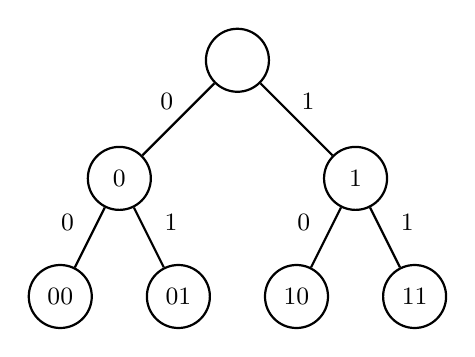
\begin{tikzpicture}[
  treenode/.style={circle,draw,minimum size=8mm,inner sep=0pt,thick,font=\small},
  edgelabel/.style={draw=none,fill=none,inner sep=8pt,font=\small},
  level 1/.style={sibling distance=30mm, level distance=15mm},
  level 2/.style={sibling distance= 15mm, level distance=15mm},
  edge from parent/.style={draw,thick}
]

% Root
\node[treenode]{}
  % left subtree
  child { node[treenode]{0} 
    child{  node[treenode]{00} 
            edge from parent node[edgelabel,near start,left] {0}
    }
    child{  node[treenode]{01} 
            edge from parent node[edgelabel,near start,right] {1}
    }
    edge from parent node[edgelabel,near start,left] {0}
  }
  % right subtree
  child { node[treenode]{1}
    child{  node[treenode]{10} 
            edge from parent node[edgelabel,near start,left] {0}
    }
    child{  node[treenode]{11} 
            edge from parent node[edgelabel,near start,right] {1}
    }
    edge from parent node[edgelabel,near start,right] {1}
  };

\end{tikzpicture}
\caption{2-ary Trie Tree}
\end{center}
\end{figure}

In the figure above, one might notice that we have labelled not just the nodes, but
also the edges of our tree. It is also possible to observe that '0' means 'descending leftways'
and '1' means 'descending leftways'. Tries have applications in the realm of string-searching (specifically web searching),
data-mining, internet routing, among others.
For the purposes of this article, we will be dealing with binary Tries whose nodes are labelled as either
'0' or '1', that is, every node of the tree will have its path from the root defined by a bitstring the size of its depth.
In order to improve readability, from now on we will refer to this structure only by Trie.

% definir associacao dos indices I_i (com figura)

We can take advatage of certain properties of this structure to yield us operations that
will prove to be useful in our algorithm.

\definition{} In a rooted tree T, the \textbf{Lowest Common Ancestor} of two nodes x and y is
the deepest node that is an ancestor of both x and y.
% \footnote{referenced from Algorithms on Strings, Trees, and Sequences
% by Dan Gusfield, \textsection 8}

To find the Lowest Common Ancestor (LCA) of two nodes in a Trie, we can simply compare the
bitstrings and find the first position where they differ, which can be calculated in constant time by using bitwise operations XOR
and CLZ (Count Leading Zeroes). For example: node x = 0001 and node y = 0011 first diverge at the third level of the
tree. In this way, given a complete \footnote{A complete Trie is a Trie where all the levels are fully filled except for the leaves}
Trie and a sequence of leaf indexes I$_0$, I$_1$, ... I$_n$, if we take the lowest common ancestor of any two indexes I$_i$ and I$_{j}$, we get the root of
the smallest subtree that contains both I$_i$ and I$_{j}$. In this way, we can calculate the LCA of every pair of adjacent indexes I$_i$, I$_{i+1}$ to
get a series of subtrees that can be used to compress our Trie by raising all leaves to their first divergence node.

\textbf{Rafael:} ainda vou colocar figuras de exemplo aqui (assim que eu aprender). Essa seção ainda não acabou.


% \textbf{Theo:} THE FOLLOWING EXPLANATION IS A TO-DO!!!! NOT FINISHED!!! THIS SEGMENT WILL MOST LIKELY NOT BE ENTIRELY FOUND HERE.

% For the purpose of our work, we apply Trie Trees to find the lowest common ancestor
% of two adjacent runs by giving each run indexes that will fit in our desired Triee Tree. 
% Our Trie Tree goes through a 'compression' step that resolves 'useless' levels, raising all
% runs to their first divergence node. This is the tree that we will use for our MergeSort algorithm
% and our merge policy will be the same as that of PowerSort, given that we have the same guarantee of
% Indexes.

\textbf{Theo:} BELOW SEGMENT IS A PLANNING LIST 

I think if we previously define Huffman Trees and how people use those trees for merges
we can segway into talking the indexes for trie-trees and compressed trees. 
Its better to work on the previous context than to continue talking about trie trees.
Trie trees are slightly novel, i think, for most people, so difining other things to compare them with
seems better than just jumping right into talking about them. 

\section{Powersort and optimality}
\textbf{Theo:} nas nossas issues, tem primeiro falar da cartesian tree e depois do powersort.
mas hmm acho que isso fica meio estranho pq o powersort que chega com 
a ideia de cartesian trees. na seção anterior ( de trie trees )
a gente pode mostrar que as trie trees garantem o limite de entropia se 
os índices forem bons sem falar de cartesiant trees e aí trazer
as cartesian trees aqui. Essa seção vai ser grande i guess
\textbf{Rafael:} acho que vale comentar pelo menos da construção sequencial da Trie comprimida
antes de seguir pro powersort, deixei essa parte pra ser a seção em que a gente faz a equivalência 
com o problema das runs.
\subsection{Trie-Tree Powersort}

\section{Mergesort Cearense}

\section{Running-Time study}

\section{Conclusion and future work}

\section{Implementations}
% OLD ARTICLE 
% \section{Definitions:}
% \textit{Clarification:} Definitions with a * at the end come from Munro and Wild's papers. This is
% a 'to-do', I will properly cite them later. 

% \textbf{Runs:} Contiguous regions of the input that are already in sorted order. 
% Let R$_0$, \dots , R$_{r-1}$ be the runs in the input, L$_i$ denotes the length of R$_i$.*

% \textbf{Run-adaptive mergesort:} Any stable run-adaptive mergesort can be described as a merge tree T: 
% an (ordered rooted) tree with leaves R$_0$, \dots, R$_{r-1}$ (appearing in that order from left to right). 
% Each internal node v of T corresponds to the result of merging its children.*

% \textbf{Merge costs:} M(v) is the total length of the resulting merge corresponding to the internal node v. 
% The total merge cost of T is then:
% \begin{equation}
% M(T) = \sum_{v \in T}M(v).     
% \end{equation}

% \textbf{Run boundaries:} Denoted by B$_i$, it is the boundary between the ($i - 1$)st and ith run (i=1, \dots, $r - 1$). 
% In binary merge trees, there is a one-to-one correspondence between the B$_i$ and the (inner/non-leaf) merge-tree nodes.*

% \textbf{Node depth:} Let d$_i$ be the depth of leaf R$_i$ in T, where depth is the number of edges on the path to the root. 
% Every element in run R$_i$ is counted exactly d$_i$ times in $\sum$$_v$M(v), so: 
% \begin{equation}
%         M = \sum^{r-1}_{i=0}d_i \cdot L_i*    
% \end{equation}

% \textbf{Node power:} Let $\alpha$$_0$, \dots, $\alpha$$_m$, $\sum$$\alpha$$_j$ = 1 be leaf probabilities. 
% For 1 $\le$ j $\le$ m, let j be the internal node separating the ($j - 1$)st and jth leaf. The power of (the split at) node j is:
% \begin{equation}
%     P_j = min\{ \ell \in N: \lfloor{\frac{a}{2^{-\ell}}}\rfloor   < \lfloor{\frac{b}{2^{-\ell}}}\rfloor \}, \text{where } a = \sum_{i=0}^{j-1} \alpha_i - \frac{1}{2}\alpha_{j-1}, b = \sum_{i=0}^{j-1} \alpha_i + \frac{1}{2}\alpha_j.
% \end{equation}

% (Pj is the index of the first bit where the (binary) fractional parts of a and b differ.)

% \textbf{Powersort:} The intuition behind Powersort is to imagine a complete binary tree T$_v$ sitting on top of 
% the array, where each element A[i] of the input corresponds to a leaf of T$_v$ .T$_v$ corresponds to the merge tree of 
% a non-adaptive two-way Mergesort (starting with individual elements). Now each run boundary B$_j$ also corresponds to an (inner) node w of 
% this (virtual) k-ary tree TV , namely the lowest common ancestor of the two leafs adjacent to B$_j$.
% *[ We need to re-explain this part better so that we can talk about the concept of a “Powersort merge tree” or something of the sorts. 
% Helps with the proof of our main proposition]  

% \textbf{Forgetful K-Stack:} A forgetful stack is a stack that forgets its k-th element if it already has k elements
% in it and a new one is added. 

% \textbf{C-Bounded Powersort:} The Powersort algorithm using a Forgetful C-Stack instead of the traditional stack with 
% size logn + 1. 

% \textbf{Processing a subtree of height h:} Let T be a merge tree, T’ one of its subtrees of size h and v the root of T’. 
% Processing T’ is executing all the merges necessary to fill node v, given that it has length M(v). 

% \section{Proofs:} 

% \textbf{Proposition:} Let T be a Powersort merge tree of height H. One pass of the C-Bounded Powersort algorithm is 
% enough to process all subtrees of T with height of C-1.

% \textit{Proof by induction:}  

% \textbf{Base case - T of height 2:}

% Let v be the root of T and v$_1$ and v$_2$ its two children. Therefore, T has two sub-trees, T’ and T’’, both of of height one. 
% For the left subtree T', v$_1$ is the root and it has only two leaf children: the runs R$_1$ and R$_2$. 
% Given that h = 1, a Forgetful 2-Stack will work with 2-Bounded Powersort as follows: 

% R$_1$  will be found and added to the stack, then, given that there is nothing to compare R$_1$  with, 
% the algorithm will search for the adjacent run, R$_2$. After finding it, the algorithm will calculate the power 
% between R$_1$ and R$_2$, which is equal to the height of v$_1$. Given that we only have one power calculated, 
% this will lead to no merges and R$_2$ will be added to our stack. Afterwards, the algorithm will proceed to the
% right T'' subtree, which is rooted in v$_2$. The algorithm will find R$_3$ and, then, calculate the power 
% between R$_2$ and R$_3$. This will result in the height of v, which is smaller than that of v$_1$, 
% our previously calculated power, leading to the merge of runs R$_1$ and R$_2$ into run R$_{12}$. 

% After this, our Forgetful 2-Stack will contain R$_{12}$ and R$_3$. Then, the algorithm will find run R$_4$. 
% Calculating the power between R$_3$ and R$_4$ leads to height v$_2$, 
% which is bigger than that of v, our previously calculated power, meaning the algorithm will not merge any 
% runs and will add R$_4$  to the Forgetful 2-Stack. This will cause the stack to “forget” about R$_{12}$, 
% meaning it will only contain R$_3$ and R$_4$. 
% Once we find R$_4$, we will have reached the end of the array. 

% Following the logic of the algorithm, once the scan reaches the end of the array everything that 
% still is in the Forgetful-Stack will be merged, thus, in this situation, a merge between R$_3$ and R$_4$ will happen,
% leading to the processing of both subtrees T’ and T’’. This concludes our base case. 

% \textbf{Hypothesis:}
% Suppose the proposition holds true for all subtrees of height h $\leq$ k in a powersort merge tree.

% \textbf{Inductive Step:} Let T be a Powersort merge tree of height H. We will prove that a (k+2)-Bounded Powersort 
% processes all of T's subtrees that have height of h = k+1. Let T' be one of those subtrees and v its root. 
% We will analyze the sub-trees T$_\ell$ and T$_r$, each rooted in the left and right children of v, v$_\ell$ 
% being the left child and v$_r$ the right child. The height of the T$_\ell$ is, at most, k, therefore, 
% we can apply our induction hypothesis and process T$_\ell$, thus, v$_\ell$ will contain run R$_\ell$, 
% which is the result of the merge of all runs in T$_\ell$. The processing of this sub-tree will happen once the 
% most-left run of T$_r$ is analyzed by the algorithm.\footnote{Once the power between the most-right run of T$_\ell$ 
% with most-left run of T$_r$ is calculated, it will result in the height of v, 
% which is smaller than the height of v$_\ell$, meaning the algorithm will merge everything left in our Forgetful k+2-Stack, 
% for all powers calculated between runs in T$_\ell$ is greater than v$_\ell$} 
% By the end of the processing of T$_\ell$, our Forgetful (k+2)-Stack will contain R$_\ell$ and
% the most-left run of T$_r$. Given that, by hypothesis, the processing of T$_r$ requires one pass of
% a (k+1)-Bounded Powersort
% \footnote{Remember that T$_\ell$ and T$_r$ have, at max, height of k}
% \footnote{Requiring a (k+1)-Bounded Powersort means the processing needs k+1 free spaces in the Forgetful C-Stack,
% not a specific tuning of the algorithm.}, and that our Forgetful (k+2)-Stack has
% exactly k spaces left, with one of them already being occupied by one run of T$_r$, 
% the algorithm will be able to process T$_r$. Similarly to what happened during the processing of T$_\ell$, 
% the calculation of the power between the right-most run of T$_r$ (which is also the right-most run of T') 
% and the next run, which is the left-most run of another subtree of T with height k+1, will result 
% in the height of v - 1.
% \footnote{This is due to the fact that both runs are in adjacent subtrees: v is the left child of a node v$_p$ and 
% there is a node v' which is the right child of the same v$_p$, the first common ancestor between v and 
% v' is v$_p$, therefore, the first common ancestor between runs in each subtree (the subtree rooted in v and 
% the subtree rooted in v') is v$_p$}. Given that all the powers calculated between runs in T' are greater than v-1, 
% the algorithm will merge all the remaining runs in our Forgetful (k+2) stack, leading to the processing of T$_r$ but 
% also to the processing of T', given that R$_\ell$ will still be on the stack alongside all runs from T$_r$. 
% Therefore, if the (k+2)-Bounded Powersort was able to process a generic T' subtree of T with height k+1, it is fair 
% to assume that it will be able to further process all the remaining subtrees of same height by following the same 
% logic as the one described for T'.
% \qed

% \newpage
% \textbf{Proposition:} It takes C-Bounded Powersort at most $\bigO(n \cdot \log{n})$ element scans to order an array of size n. 
% \begin{proof}
% Each pass through the array scans element i, with 0 $\leq$ i $\leq$ n, at least once. Given that the algorithm will 
% do $\frac{\log{n}}{c-1}$ passes\footnote{The height of a Powersort merge tree T is $\log n$ and the C-Bounded Powersort
% algorithm starts by processing subtrees of T that have height less than or equal to c-1. 
% This results in a smaller tree T' of height $\log n$ - (c-1). A second pass will, once again, 
% process the subtrees of T' that have height less than or equal to c-1, resulting in a smaller tree T''. 
% Therefore, if k is the amount of trees created by this process until the last tree is of height less than or equal to c-1, 
% meaning it will only require one last pass of the algorithm to be processed, k$\cdot$(c-1) $\leq$ $\log n$}, i will be read
% at least $\frac{\log{n}}{c-1}$ times. Once the entire array is ordered, i will also have been read at least twice 
% for each merge it was present in, i.e, 2$\cdot$d$_i$, with d$_i$ being equal to the height of T. Therefore,
% the total number of scans is:
% \begin{equation}
% Scans \leq \sum^{n}_{i=0}2\cdot \log{n} + n \cdot \frac{\log{n}}{c-1}
% \end{equation}
% \begin{equation}
% Scans \leq n\log{n}\cdot(2 + \frac{1}{c-1})
% \end{equation}
% \begin{equation}
% Scans \leq \bigO(n \cdot \log{n})
% \end{equation}
% \end{proof} 
% \newpage

% \section{Pseudocodes:}
% \noindent\textbf{TO-DOs:} \newline
% \noindent 1. Os comentários para cada algoritmo precisam estar de acordo com as definições usadas
% no primeiro esboço do artigo (powersort.tex) e precisam ser revisados para fazerem
% sentido, alguns ainda estão bem abstratos e/ou não descrevem corretamente os algoritmos. \newline
% \noindent 2. Tanto para esse pdf quanto para o anterior, ou seja, para o artigo como um todo, o nome do professor Victor se enquadra como autor? Imagino que sim.
% Essa pergunta é meio boba. \newline
% \noindent 3. Código para a estrutura de dados que iremos usar. \newline
% \noindent 4. Reestruturar o vai e volta. \newline
% \noindent\textbf{Planejamento da estrutura:} Guardaremos o início da primeira run, seu fim e seu power com a run anterior (se houver), além disso,
% cada elemento seguinte será: o fim da run e o power da run com a anterior. 
% run e não teremos um elemento sentinela. O inicio de uma run baseia-se no fim da anterior + 1. Assim que incluimos um elemento
% que estoura o tamanho da pilha, temos que esquecer o primeiro elemento e ajustar
% o novo primeiro elemento para também guardar o seu início.
% (cada pop ou insert decrementa ou aumenta o tamanho) 

% \noindent Como vamos fazer scans da esquerda para a direita e da direita para a esquerda, precisamos 
% alternar entre somar um no fim de uma run para achar o começo da próxima e diminuir um. $\gets$ pensar nisso

% \noindent \textbf{Comentário do professor:} ``{Só um detalhe de notação, usa aqui (A, s$_2$, n). A[s$_2$] é o valor e não o índice.}''

% \noindent \textbf{Resposta:} Fiz desse jeito porque é a forma que eles escreveram no artigo, mas achei bem estranho também, depois vou mudar.



% \noindent \textbf{Introduction:} We are very smart and we know things, this is the complaints we have for things
% that weren't done by us and how we would have made them better. 
% \newpage
% \subsection{Powersort Versions:}
% \subsubsection{\textbf{Standard Powersort}}
% \textbf{Commentary on Wild and Munro's version:} 
% A single pass algorithm that sorts the entire array. 
% \begin{algorithm}
% \caption{Powersort(A[1...n]) by Wild and Munro:}
% \begin{algorithmic}[1]
% \State $X :=$ stack of runs \Comment{capacity $\lfloor{lgn(n)}\rfloor + 1$}
% \State $P :=$ stack of powers \Comment{capacity $\lfloor{lgn(n)}\rfloor + 1$}
% \State $s_1 := 1; e_1 = ExtendRunRight(A[1], n)$
% \While{$e_1 < n$}
%     \State $s_2 := e_1 + 1; e_2 := ExtendRunRight(A[s_2], n)$ \Comment{A[$s_2..e_2$] next run}
%     \State $p := NodePower(s1, e1, s2, e2, n)$ \Comment{$P_j$ for node j between A[$s_1..e_1$] and A[$s_2..e_2$]}
%     \While {P.top() $>$ p} \Comment{previous merge deeper in tree than current}
%         \State P.pop() \Comment{$\rightarrow$ merge and replace run A[$s_1..e_1$] by result}
%         \State ($s_1, e_1$) := Merge(X.pop(), A[$s_1..e_1$])
%     \EndWhile \State X.push(A[s1, e1]); P.push(p)
%     \State $s_1 := s_2; e_1 := e_2$
% \EndWhile 
% \State \textbf{end while} \Comment{Now A[$s_1..s_1$] is the rightmost run}
% \While{¬X.empty()}
%     \State ($s_1, e_1$) := Merge(X.pop(), A[$s_1..e_1$])
% \EndWhile 
% \end{algorithmic}
% \end{algorithm}
% \newpage
% \subsubsection{\textbf{\textbf{First variation of C-Bounded Powersort (only goes right)}}}
% \textbf{Commentary on our first version:} 
% This algorithm performs multiple passes on the array, processing all subtrees
% of height C-1 with each pass. We remind the reader of how Powersort works:
% It is implicitly a complete binary tree of size $\log{n}$. Therefore, the max amount of passes
% needed to sort the array is:
% \begin{equation}
%     \text{N° of scans} \leq {\frac{\log{n}}{{C-1}}}
% \end{equation}
% \begin{algorithm}
% \caption{C-Bounded-Powersort 1(A[1...n], C):}\label{alg:powermy1}
% \begin{algorithmic}[1]
% \State $X :=$ C-bounded stack of runs \Comment{capacity C}
% \State $P :=$ C-bounded stack of powers \Comment{capacity C}
% \State $s_1 := 1; e_1 = ExtendRunRight(A[1], n)$
% \While{$e_1 < n$} \Comment{{\small This while can be tweaked to use max amount of passes}}
%     \While{$e_1 < n$} \Comment{A single pass goes until the end of the array}
%         \State $s_2 := e_1 + 1; e_2 := ExtendRunRight(A[s_2], n)$
%         \State $p := NodePower(s1, e1, s2, e2, n)$ \Comment{{\small Using our node power algorithm}}
%         \While {P.top() $>$ p} \Comment{We follow the same merge policy}
%             \State P.pop()
%             \State ($s_1, e_1$) := Merge(X.pop(), A[$s_1..e_1$])
%         \EndWhile \State X.push(A[s1, e1]); P.push(p)
%         \State $s_1 := s_2; e_1 := e_2$
%     \EndWhile 
%     \State \textbf{end while}
%     \While{¬X.empty()}
%         \State ($s_1, e_1$) := Merge(X.pop(), A[$s_1..e_1$]) 
%     \EndWhile 
%     \State \Comment{{\small We're using a limited stack, so we need to check for another pass}}
%     \State $s_1 := 1; e_1 = ExtendRunRight(A[1], n)$ \Comment{{\small If $e_1$ = end, the array is sorted}}
% \EndWhile 
% \State \textbf{end while}
% \end{algorithmic}
% \end{algorithm}
% \newpage
% \noindent\textbf{After first modifications:}
% \subsubsection{\textbf{\textbf{Second variation of C-Bounded Powersort (goes left and right!)}}}
% \textbf{Commentary on our second version:} This works rather similarly to our first version.
% The main difference is the fact that, once we reach the end of the array, instead of restarting
% our scan from the beginning, we scan, starting from the end, to the left, until we reach the beginning of the array,
% and, thus, we repeat the scan-right process.
% This is slightly better than the first version, given that it takes advantage of 
% runs still being in cache instead of restarting from the beginning.

% \noindent\textbf{Comentário sobre X.size \textgreater 1:} Ao invés de termos uma stack X e P, teremos somente uma Stack guardando power e runs. 
% Assim, caso mantenhamos uma run dentro da stack após o final de um scan, ela não estará com o 'power' correto quando
% o próximo scan iniciar. Isso significa que teríamos que dar um pop nessa pilha e tratá-la como vazia. Podemos fazer um s1 $\gets$ top,
% visto que a run a ser achada por e$_1$ := ExtendRunSide depois de um scan vai ser sempre a run resultante de todos os merges finais (será?)
% %para o código quebrar páginas, não podemos usar o algorithm, logo, fiz um template de header

% \noindent\rule{\linewidth}{0.8pt}\par % linha preta do topo para fazer um header
% \vspace{-0.3em} % espaçamento 
% \noindent\textbf{Algorithm 3} C-Bounded-Powersort 1(A[1...n], C):\label{alg:powermy2temp}

% \vspace{-0.6em} % espaçamento
% \noindent\rule{\linewidth}{0.5pt}\par % linha preta de baixo para fechar o header
% \vspace{-0.5em} % espaçamento
% \begin{algorithmic}[1]
% \State $X :=$ C-bounded stack of runs and powers
% \State $s_1 := 1; e_1 = ExtendRunRight(1, n)$
% \While{$true$}
%     \If{$e_1 == n$}
%     \State break
%     \EndIf
%     \While{$e_1 < n$} 
%         \State $s_2 := e_1 + 1; e_2 := ExtendRunRight(s_2, n)$ 
%         \State $p := NodePower(s1, e1, s2, e2, n)$
%         \While {X.size \textgreater \text{ }1 and X.top().power $>$ p}
%             \State ($s_1, e_1$) := Merge(X.top().boundary, A[$s_1..e_1$])
%             \State X.pop()
%         \EndWhile \State X.push(s1, p);
%         \State $s_1 := s_2; e_1 := e_2$
%     \EndWhile
%     \State \textbf{end while} 
%     \While{$X.size > 1$}
%         \State ($s_1, e_1$) := Merge(X.pop(), A[$s_1..e_1$]) 
%     \EndWhile
%     \State $s_1 := n; e_1 = ExtendRunLeft(A[n], 1)$ \Comment{{\scriptsize Now, we're scanning from right to left!}}
%     \If{$e_1 == 1$}
%         \State break \Comment{{\scriptsize If we could extend until the beginning, our run is the entire array.}}
%     \EndIf
%     \While{$e_1 > 1$} \Comment{We're scanning from n down to 1}
%         \State $s_2 := e_1 - 1; e_2 := ExtendRunLeft(s_2, 1)$ 
%         \State $p := NodePower(s1, e1, s2, e2, n)$
%         \While {X.size \textgreater \text{ }1 and X.top() $>$ p}
%             \State ($s_1, e_1$) := Merge(X.top().boundary, A[$s_1..e_1$])
%             \State X.pop()
%         \EndWhile \State X.push(s1, p); 
%         \State $s_1 := s_2; e_1 := e_2$
%     \EndWhile 
%     \State \textbf{end while}
%     \While{$X.size > 1$}
%         \State ($s_1, e_1$) := Merge(X.pop(), A[$s_1..e_1$]) 
%     \EndWhile
%     \State $s_1 := 1; e_1 = ExtendRunRight(1, n)$ \Comment{{\small Now, we're scanning from left to right!}}
% \EndWhile
% \end{algorithmic}
% \vspace{-1em}
% \noindent\rule{\linewidth}{0.5pt}\par 

% \subsection{NodePower versions:}
% \subsubsection{Standard Nodepower:}
% \textbf{Commentary on Wild and Munro's Node Power:} This is so silly and expensive! 

% \noindent\rule{\linewidth}{0.8pt}\par
% \vspace{-0.3em} 
% \noindent\textbf{Algorithm 4} NodePower($s_1,e_1,s_2,e_2,n$):\label{alg:nodepower1}

% \vspace{-0.6em} 
% \noindent\rule{\linewidth}{0.5pt}\par 
% \vspace{-0.5em} 
% \begin{algorithmic}[1]
% \State $n_1 := e_1 - s_1 + 1;$ \text{ } $n_2 := e_2 - s_2 + 1;$ \text{ } $\ell := 0$
% \State $a := (s_1 + n_1/2 - 1)/n;$ \text{ } $b := (s_2 + n_2/2 - 1)/n$
% \While{$\lfloor a \cdot 2^\ell \rfloor == \lfloor b \cdot 2^\ell \rfloor$ \textbf{do} $\ell := \ell + 1$ \textbf{end while}}
% \EndWhile   
% \State \textbf{return ($\ell$)}
% \end{algorithmic}
% \vspace{-1em} 
% \noindent\rule{\linewidth}{0.5pt}\par 

% \subsubsection{Our Nodepower:}
% \textbf{Commentary on our Node Power:} Ours is cool and epic.
% (TO-DO: explanation of why it works)

% \noindent\rule{\linewidth}{0.8pt}\par 
% \vspace{-0.3em} 
% \noindent\textbf{Algorithm 5} NodePower($s_1,e_1,s_2,e_2,n$):\label{alg:nodepower2}

% \vspace{-0.6em} 
% \noindent\rule{\linewidth}{0.5pt}\par 
% \vspace{-0.5em} 
% \begin{algorithmic}[1]
% \State xor $:= s_1$ \textbf{\^{}} $s_2$
% \State first\_{}bit := \_{\_{}}builtin\_{}clz(xor)
% \State $\ell :=$ first\_{}b
% \State \textbf{return ($\ell$)}
% \end{algorithmic}
% \vspace{-1em}
% \noindent\rule{\linewidth}{0.5pt}\par
% \newpage
% \subsection{The data structure:}
% \textbf{Introduction:} Wild and Munro's paper shows no specific code for their stack data structure,
% this is probably due to the fact that they simply use a standard stack of height $\log n$.
% Thus, we will have no 'counterpart' algorithm to analyze. Our algorithm implements a modified version of a stack which
% we call "C-Bounded Stack"/"Forgetful Stack".

% \subsubsection{C-Bounded Stack:}
% \noindent\textbf{Commentary on our data structure:} 
% When creating this data structure, we had to think of two particularities:

% \noindent \textbf{1}. This is a stack of limited size.

% \noindent \textbf{2}. This is a stack that has to consider scans going right and a scans going left.


% \noindent In order to deal with the limited size, which is the 'forgetful' aspect of the data structure,
% we simply use circularity: we keep the index of where the next new element will be inserted in the case of a push and
% increment it. If we reach the end of the array, we assign the free space to be the first element and overwrite it in case of a push.
% As the stack fills, we also increment a variable for 'size', which corresponds to the amount of elements in the stack. 
% Thus, we keep two variables, one for 'top' and one for 'size'. Other than that, each element in the stack consists
% of a run boundary and the power of this run with its predecessor.

% \noindent\textbf{Run boundaries:} When the algorithm is scanning right, the boundary it keeps is the start of the run found. 
% When the algorithm is scanning left, the boundary it keeps is the end of the run found.

% \noindent\rule{\linewidth}{0.8pt}\par
% \vspace{-0.3em} 
% \noindent\textbf{Algorithm 6} C-Bounded Stack(initial run $s_1$, size C):\label{alg:stack}

% \vspace{-0.6em} 
% \noindent\rule{\linewidth}{0.5pt}\par 
% \vspace{-0.5em} 
% \begin{algorithmic}[1]
% \State top := 1
% \State size := 0
% \State MaxSize := C
% \State array[MaxSize]
% \State \textbf{func Pop()}\{
% \If{size \textgreater \text{ } 1:}
%     \If{top == 1:}
%     \State top $\gets$ MaxSize
%     \Else
%     \State top$--$ 
%     \EndIf
%     \State C$--$ \}
% \EndIf
% \State \textbf{func Push(\textnormal{run boundary$_i$, power k})}\{
% \State array[top] $\gets$ (boundary$_1$, k)
% \State top $\gets$ top\%MaxHeight + 1
% \If (C $\neq$ MaxHeight:)
% \State C$++$ 
% \EndIf \}
% \State \textbf{func Top()}\{
% \If {C $\geq$ 1:}
% \State return array[(top == 1) ? MaxHeight : (top - 1)] \}
% \Else 
% \State return null
% \EndIf
% \end{algorithmic}
% \vspace{-1em} 
% \noindent\rule{\linewidth}{0.5pt}\par 

% \printbibliography	

\end{document}